\section{Detection and Measurement of REE concentration\authorA{}}

%Rare Earth Elements (for short: REEs) play a critical role in modern-day life.
%They are used in nearly every device that uses electrical power to operate.
%A few example where REEs are essential are: lasers, computer monitors, electric motors, high-power magnets, liquid crystal displays (LCDs), solar panels~\cite{usageofrees}.
%In this context, it is clear that the demand for REEs is rising rapidly.
%In the following years, with more and more electronic devices produced, most of them will eventually end as electronic waste.
%Recycling REEs from this waste is crucial for the worlds REE supply.
%Current recycling methods are mostly harmful to the environment and very costly~\cite{recyclingcurrent}.
%But new recycling methods have emerged in the last years and one of them, using the technique of biosorption, is the subject of this thesis.
%To understand how this process works, it is important to know the following techniques.

The detection of rare earth elements in a sample is a crucial step in our work.
It allows us to quantify the effectiveness of our process.

In modern chemistry,
qualitative and quantitative analysis of elements in a sample is usually done with inductively coupled plasma mass spectroscopy (ICP-MS) or atom absorption spectroscopy (AAS).
However, as the ICP-MS and AAS use machines that are very, very expensive,
these methods were not an option as they exceeded our limited financial resources by far.
Instead, we had to search for other methods to detect and quantify rare earths.

In our work, we used two precipitation reactions and one method to quantify the concentration of REEs.


\subsection{Precipation Reactions}

\subsubsection{Cer Precipitation Reaction}
The precipitation reaction for cer works by utilizing the oxidation states +III and +IV~\cite{cerdetection,janderblasius}.

\begin{figure}[H]
    \centering
    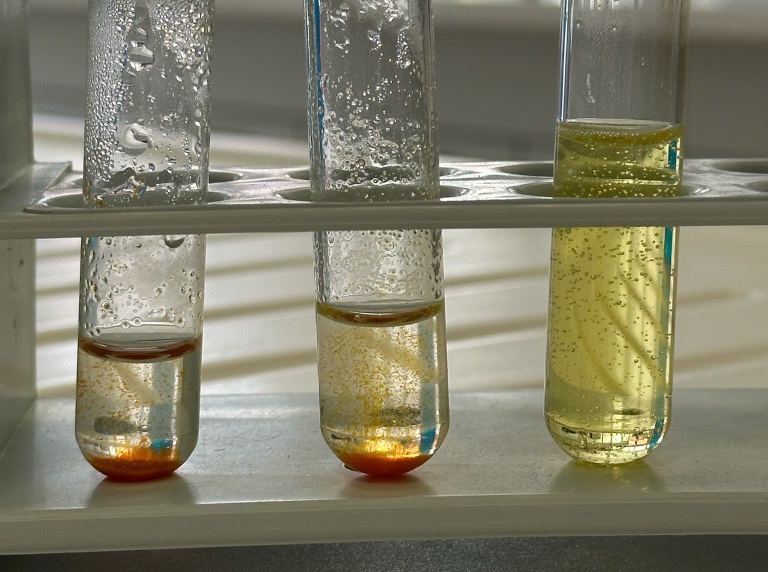
\includegraphics[width=0.9\textwidth]{./media/images/ree_precipitation_reaction_cropped}
    \caption{Precipitation of a successful cer detection reaction. The test tube on the righthandside does not show any precipitation because the sample was deionized water.}
    \label{fig:cer_precipitation_cropped1}
\end{figure}

Cer in the aforementioned states forms complexes together with \ce{H2O2}.
The complexes are called cer peroxide hydrates.
Their chemical formulas are \ce{Ce(OH)2(OOH)} and \ce{Ce(OH)3(OOH)}.
These complexes fall out of the solution as a red-brown colored precipitate.

\subsubsection{Neodymium Precipitation Reaction}
The reaction to detect neodymium is a bit more complicated.
It also uses the +III oxidation state of neodymium.
The neodymium reacts with acetic acid to form neodymium acetate.
As the last step, iodide is given to the solution which forms a blue-colored complex together with the neodymium acetate~\cite{janderblasius}.

\begin{figure}[H]
    \centering
    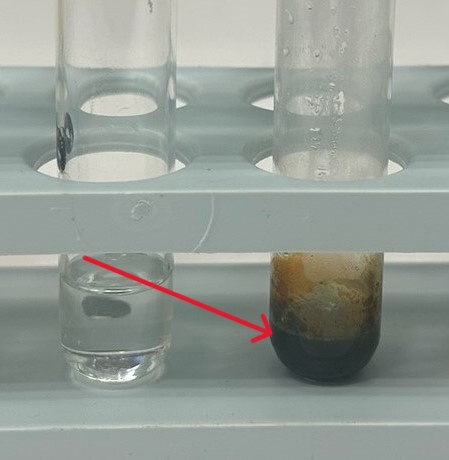
\includegraphics[width=0.9\textwidth]{./media/images/nd_precipitation_reaction_cropped}
    \caption{Neodymium detection reaction. Neodymium is contained in the sample of the third test tube (left to right). The blue precipitate is clearly visible.}
    \label{fig:nd_precipitation}
\end{figure}

\newpage


\subsection{Arsenazo III Assay}

\subsubsection{Arsenazo III}
The arsenazo III assay is based on the dye arsenazo III or ASIII~\cite{arsenazo3assay}.
It is often used to detect calcium, uranium and a lot of other metals, including rare earth elements~\cite{arsenazo3usage, arsenazo3othermetals}.

\begin{figure}[H]
    \centering
    \chemfig[bond style={line width = 1pt}, double bond sep = 3pt]{*6((-S(=[3]O)(=[7]O)-HO)-=(*6(-=(-S(=[1]O)(=[5]O)-OH)-(-N(=[2]N-(*6(=-=-=(-As(=[5]O)(-[1]OH)-HO)-))))=(-OH)--))-=(-OH)-(-N(=[2]N-(*6(=(-As(=[7]O)(-[3]HO)-OH)-=-=-))))=)}
    \caption{Structure of 2,7-bis(2-arsenophenylazo)-1,8-dihydroxynaphthalene-3,6-disulfonic acid. Or, in its abbreviated form, arsenazo III.}
    \label{fig:asiii_structure}
\end{figure}

Arsenazo III was first synthesized in 1959~\cite{arsenazo3fortyyears}.
In comparison to arsenazo I and II, it possesses two functional arseno groups (see fig.~\ref{fig:asiii_structure}).
The arsenazo III dye has the property to change its color based on the pH and the presence of some elements.
Normally, the dye has a pinkish-crimson color, but when, for example, thorium is present, the color changes to green.
For other elements, other colors have been reported, such as blue for calcium or violet-blue and also green for rare earth elements.

\begin{figure}[H]
    \centering
    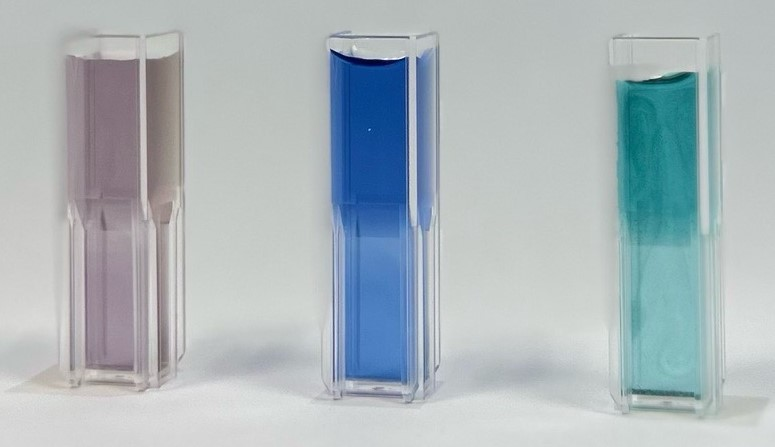
\includegraphics[width=0.9\textwidth]{./media/images/asiii_color_change}
    \caption{Example for different colors of arsenazo III with different samples. The contents of the cuvettes are (from left to right): \ce{FeCl3}, \ce{CuSO4}, \ce{NdCl3}. All are mixed with 10µL of 10mM arsenazo III.}
    \label{fig:asiii_colors}
\end{figure}

The color change happens, because the arsenazo III forms complexes with certain elements.
Arsenazo III and rare earths and some other metals form 1:1 complexes~\cite{arsenazo3complex, arsenazo3structurecomplex}.
This means that for every molecule of arsenazo III, one rare earth element atom was bound (see fig.~\ref{fig:asiii_complex_structure}).
The other arseno group is most likely not used to form these stable complexes.


\begin{figure}[H]
    \centering
    \schemestart
    \chemfig[atom sep = 4em, bond style={line width = 1pt}, double bond sep = 3pt]{[:120]*6(-[,,,,dash pattern = on 10pt off 10pt]=(-O?[a])-(-[3]N(=[2]N@{a1}-(*6(=(-As(=[2]O)(-[7,0.7]OH)-O(-[:300,1.5,1,3,dash pattern = on 2pt off 2pt]@{a2}REE?[a,1,{dash pattern = on 2pt off 2pt}]))-[,,,,dash pattern = on 10pt off 10pt]=[,,,,draw=none]-[,,,,draw=none]=[,,,,draw=none]-[,,,,dash pattern = on 10pt off 10pt]))))=[,,,,dash pattern = on 10pt off 10pt])}
    \schemestop
    \chemmove[shorten <=4pt,shorten >=4pt]{
    \draw(a1)..controls +(45:8mm) and +(215:8mm)..(a2);
    \draw(-1,5.7) rectangle (-2.05,6.25);
    }
    \caption{An arsenazo III complex with an atom of a rare earth element.}
    \label{fig:asiii_complex_structure}
\end{figure}


\subsubsection{Probe Preparation}
To get reliable and correct results, the sample must be prepared beforehand.
This happens by adjusting the pH level of the sample solution to around 2.7 to 2.8.
This ensures that only rare earth ions interact with the arsenazo III dye.
Another advantage of this acidic level is that the ions of the rare earths dissolve better from the sample.

\subsubsection{Measuring REE Concentration}
The measuring of the concentration of the rare earths works with a UV-Vis-spectrometer.
This is a device, that can produce light with a single wavelength.
The light goes through the sample and the light intensity is measured.
When the intensity of the outgoing light \(I\) is set in relation to the intensity of the ingoing light \(I_0\), the emerging result is the transmittance \(T\)~\cite{transmittanceformula}.
\[T=\frac{I}{I_0}\]
The transmittance is then used to calculate the absorbance \(A\) using the following formula~\cite{arbsorbanceformula}.
\[A=\log{T^{-1}}=\log{\frac{I_0}{I}}\]
The absorbance is the output of the UV-Vis-spectrometer.
It is possible to measure just the absorbance at one single wavelength with the device.
However, it can also measure the absorbance from a series of wavelengths and plot the result to a spectrum.
For the Arsenazo III assay, the absorbance at the wavelength of around 650 nm is important (see fig.~\ref{fig:example_spectrum}).
\begin{figure}[H]
    \centering
    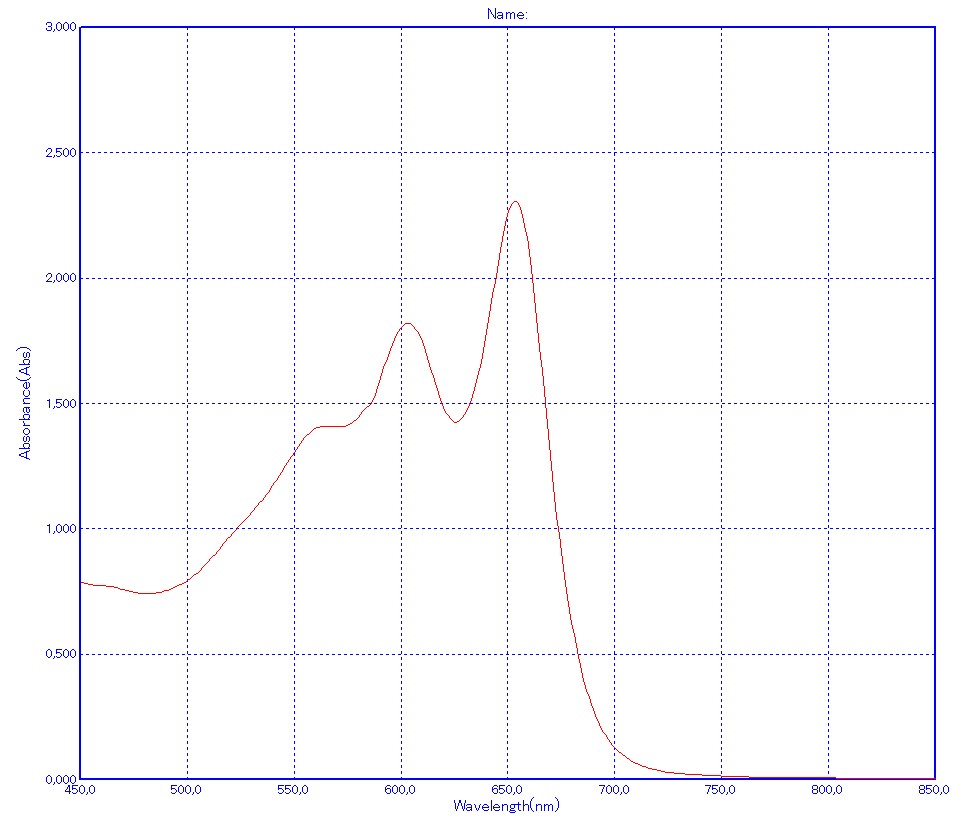
\includegraphics[width=0.9\textwidth]{./media/images/example_spectrum}
    \caption{Example of a spectrum of an arsenazo III assay. The peak at around 650nm is the product of a complex formed by one rare earth atom and one arseno group.}
    \label{fig:example_spectrum}
\end{figure}

The final measurement is done with a 1 mL cuvette.
Half of it is filled with a phosphate-citrate buffer to ensure a correct pH level.
Afterwards, 490 µL of the sample and 10 µL of the Arsenazo III dye are added to the cuvette.
The solutions in the cuvette have to be mixed, and then a spectrum from 500 nm to 800 nm is recorded.
The absorbance at 650 nm is noted.
This is later used for calculation of the concentration.
Then, 20 µL of Arsenazo III are again added and mixed into the cuvette.
The spectrum and the value at the wavelength of 650 nm are again recorded.
The dual measurement is necessary for rare earth concentrations of more than 2µmol/L, because it was found that these values suit better for higher concentrations.

These measurements are not only done with the samples but also with solutions that contain a known concentration of rare earths.
The values can then be used to calculate a calibration line which in turn gives us the concentration of the samples.